\section{Der naive Algorithmus}
Ein naheliegender Ansatz zur viewshed Berechnung ist, für jeden Punkt $p$ im DEM einzeln die Sichtbarkeit zu bestimmen. 
Dazu werden die Punkte bestimmt, die von der Strecke $sp$ zwischen dem Standpunkt $s$ und dem aktuellen Punkt $p$ geschnitten werden. Ein Beispiel für eine derartige Strecke und die davon geschnittenen Punkte ist in Abbildung~\ref{naive_p} dargestellt. 

\begin{figure}[!ht]
 \centering
 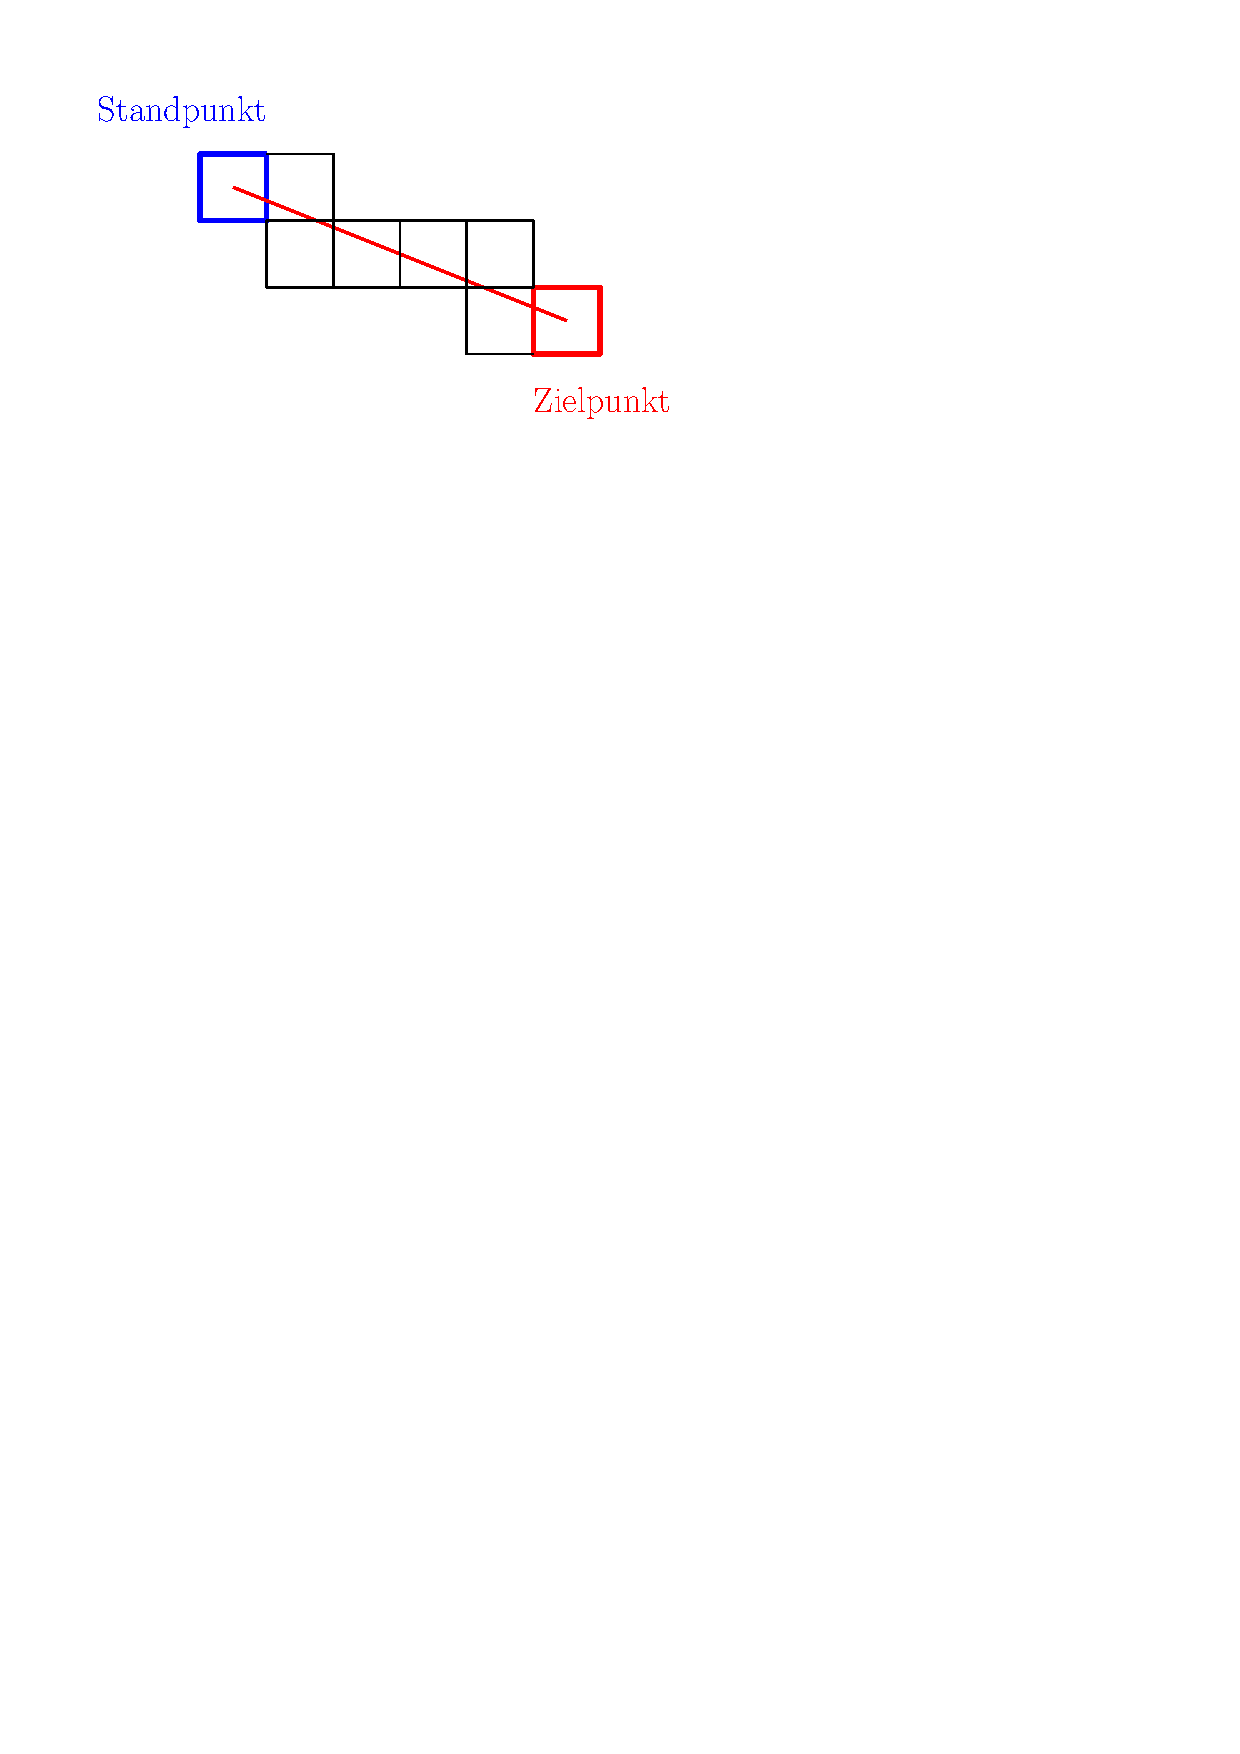
\includegraphics[scale=0.55]{../graphics/naive}
 \caption{Darstellung der geschnittenen Punkte zwischen dem Standpunkt und dem aktuellen Punkt}
 \label{naive_p}
\end{figure} 

Mithilfe dieser Punkte lässt sich bestimmen, ob $p$ sichtbar ist; Sofern ein geschnittener Punkt höher als die Verbindungslinie ist, ist $p$ nicht sichtbar. In unserer Implementation wurde die Steigung zwischen dem Standpunkt und Punkt $p$ berechnet und verglichen. Falls einer der geschnittenen Punkte eine größere Steigung als der zu überprüfende Punkt $p$ aufweist, ist dieser nicht sichtbar. Die Vorgehensweise ist in Abbildung~\ref{pseudo:naiv} in Pseudocode dargestellt. 

Die Ausgabe des Algorithmus ist ein zweidimensionales boolean Array, dass die Sichtbarkeit angibt. Die Ausgabe unseres Programms erfolgt wahlweise als PNG-Grafik oder als ASCII-Grid Daten (analog Abbildung~\ref{testfile}).



\begin{figure}[!ht]
 \centering
 \begin{BVerbatim}
 Gegeben: Standpunkt s, DEM d
 foreach Punkt p in d
    Do 
        Bestimme Punkte die von der Strecke sp geschnitten werden 
        Berechne die Steigung zwischen s und geschnittenen Punkten
        Wenn max(Steigung geschnittener Punkte) < Steigung s nach p
            p ist sichtbar
        sonst
            p ist nicht sichtbar
    EndDo
\end{BVerbatim}
\caption{Pseudocode für den naiven Ansatz}
\label{pseudo:naiv}
\end{figure}

Die Laufzeit dieses Algorithmus liegt in $O(n^3)$, wobei $n$ hierbei für das Maximum der Breite/Höhe des gegebenem DEMs ist. 
Die Größe der Ein- und Ausgabe und der zu überprüfenden Punkte liegt somit in $O(n^2)$. 
Für jeden dieser Punkte müssen die Punkte bestimmt werden, die geschnitten werden. Die Anzahl dieser liegt in $O(n)$. 
Für alle geschnittenen Punkte muss jeweils die Steigung berechnet und das Maximum ermittelt werden. Pro Punkt wird dafür konstante Zeit benötigt. 
Auch der Vergleich zwischem der Steigung von dem Maximum und des aktuellen Punktes benötigt $O(1)$ Zeit. 
Insgesamt benötigt der Algorithmus somit $O(n^3)$ Zeit für die Berechnung des viewsheds.